\section{Experimental and Theoretical Setup}
The experimental realization of such collision events is a highly challenging problem itself. The two most known colliders focusing on different aspects of relativistic heavy-ion collisions are on the one hand the \enquote{\textbf{R}elativistic \textbf{H}eavy-\textbf{I}on \textbf{C}ollider} (RHIC) at the Brookhaven National Lab in the USA studying various areas of high-energy nuclear physics for example the spin structure of the proton and as mentioned before the physics of the QGP at center-of-mass energies of about $\sqrt{s}=500$ GeV and on the other hand the \enquote{\textbf{L}arge \textbf{H}adron \textbf{C}ollider} (LHC) at CERN in Geneva, or more precisely the ALICE experiment at the LHC which is specialized on the analysis of Pb-Pb collision events at even higher center-of-mass energies of $\sqrt{s}=5.02$ TeV. We won't go into detail here concerning the exact experimental setup, the interested reader is invited to visit the corresponding websites of the experiments for more information and pictures. \\

\noindent 
The central goal of our discussion is to understand how the partons freed in relativistic heavy-ion collisions thermalize. The relevant quantity serving as an input for the subsequent hydrodynamical description is the energy-momentum tensor $T^{\mu\nu}$. We are therefore interested in its exact form and evolution. Since we are dealing with a high-energy experiment the relevant parton contribution is dominated by gluon saturation and occupation numbers of the order of $\sim 1/\alpha_{\mathrm{s}}$, where $\alpha_{\mathrm{s}}$ denotes the strong coupling constant. One refers to this state characterized by the fact that the chromo-electric and chromo-magnetic fields are collinear to the collision axis as \enquote{Glasma}. The theoretical model suitable for a description of this situation immediately after the collision is the so-called \enquote{\textbf{C}olor-\textbf{G}lass \textbf{C}ondensate} effective field theory (CGC). \newpage
\begin{figure}[t]
	\centering
	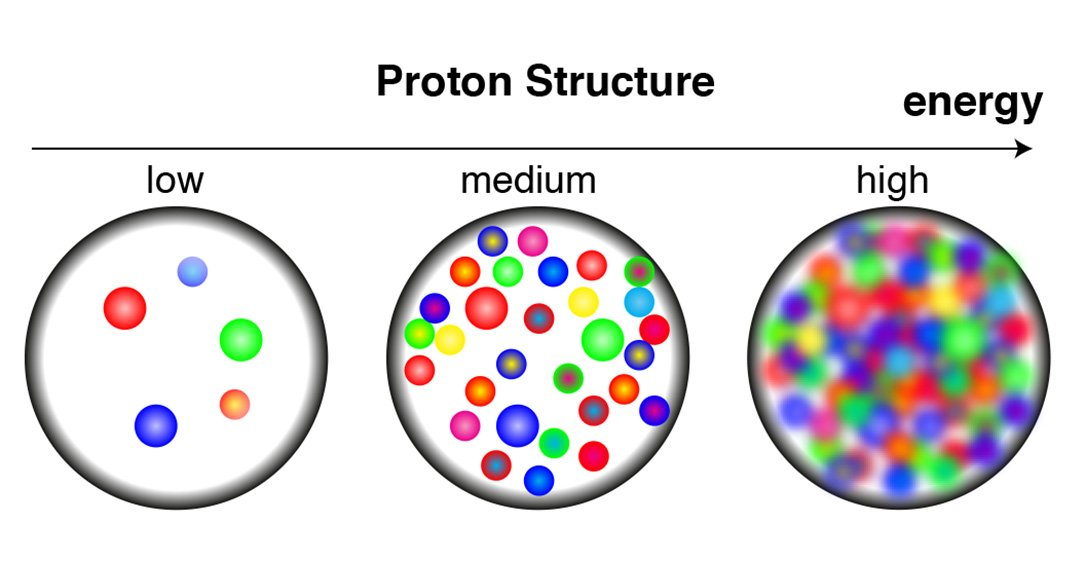
\includegraphics[width=0.6\textwidth]{figures/cqc}
	\caption[Visualization of the Color-Glass Condensate model.]{Visualization of the Color-Glass Condensate model.\footnotemark}
	\label{fig:cgc}
\end{figure}
\footnotetext{Figure taken from: \tiny\url{https://www.uu.nl/en/research/institute-for-subatomic-physics/research/color-glass-condensate} (29.06.2020)}
\noindent
As visualized in figure \ref{fig:cgc} above, the gluon density increases rapidly for high energies until the resolution is saturated at some energy scale $Q_{\mathrm{s}}$ providing a natural cutoff for the validity of the CGC model. The observation that we are dealing with very high gluon densities and therefore a highly packed phase space in this limit leads us to the conclusion that the high-$p$ states are also occupied resulting in a small coupling constant $\alpha_{\mathrm{s}} \ll 1$ due to asymptotic freedom as characteristic property of QCD.\\
The corresponding energy-momentum tensor takes the rather simple diagonal form 
\begin{equation}
	 T^{\mu\nu}_{\mathrm{Glasma}}= \operatorname{diag}(\varepsilon,\varepsilon,\varepsilon,-\varepsilon).
\end{equation}
The minus sign in the last component signals a negative longitudinal pressure at early times which is causing problems with the usability of this explicit energy-momentum tensor as an initial parameter of the hydrodynamical evolution. One expects this situation to change rapidly on a time scale $\sim 1/Q_{\mathrm{s}}$.\\
But even if this change occurs we cannot be completely sure if at all and under which conditions the expected equilibrium distribution, given by the well-known Bose-Einstein distribution 
\begin{equation}
	f_{\mathrm{eq}}(\mathbf{k}) = \frac{1}{\exp(\frac{\omega_{\mathbf{k}}-\mu}{T}) - 1}, \label{eqn:BEdist}
\end{equation}
is reached at the end of the thermalization process. Here $\omega_{\mathrm{k}}$ denotes the energy of a gluon with momentum $\mathrm{k}$, $\mu$ is the chemical potential and $T$ is the equilibrium temperature. \\

\noindent
To conclude our study of the initial situation of the collision event we have to take a look at the population of the QGP based on the CGC description presented before. The gluons have typical transverse momenta of the order of $Q_{\mathrm{s}}$ and an energy density of 
\begin{equation}
	\varepsilon_0 = \varepsilon(\tau=Q_{\mathrm{s}}^{-1})\sim \frac{Q_{\mathrm{s}}^{4}}{\alpha_{\mathrm{s}}},
\end{equation}
the number of gluons per unit volume is 
\begin{equation}
	n_0 = n(\tau=Q_{\mathrm{s}}^{-1})\sim \frac{Q_{\mathrm{s}}^{3}}{\alpha_{\mathrm{s}}},
\end{equation}
and therefore we indeed find $\varepsilon_0/n_0 \sim Q_{\mathrm{s}}$ for the average energy per gluon. The initial distribution may be characterized by the dimensionless combination
\begin{equation}
	n_0\cdot\varepsilon_0^{-3/4}\sim \frac{1}{\alpha_{\mathrm{s}}^{1/4}}.
\end{equation}
For the expected equilibrium distribution at temperature $T$ we know
\begin{equation}
	\varepsilon_{\mathrm{eq}} \sim T^{4},\qquad n_{\mathrm{eq}} \sim T^{3}
\end{equation}
and therefore 
\begin{equation}
	n_{\mathrm{eq}}\cdot\varepsilon_{\mathrm{eq}}^{-3/4}\sim 1,
\end{equation}
leaving a mismatch by a large\footnote{Remember we are working in small coupling asymptotics ($\alpha_{\mathrm{s}} \ll 1$) due to the occupation of the high-momentum states and asymptotic freedom.} factor of $\alpha_{\mathrm{s}}^{-1/4}$ corresponding to an \enquote{overpopulation} of the initial distributions.\\
\noindent
In the following we want to make use of a bottom-up approach to resolve this problem and to understand the thermalization process, i.\,e. we assume that the relaxation occurs as a result of hard elastic and inelastic collisions based on the work published in \cite{Blaizot2012, Blaizot2016}.
